\subsection{Architectuur}
\label{subsec:architectuur}

De applicatiearchitectuur die Canvas.hs gebruikt bestaat uit drie componenten. De applicatie van de gebruiker, de Canvas.hs module en de JavaScript Canvas.hs applicatie—in dit verslag aangeduid als de client. De module en de client vormen samen de Canvas.hs library.

De Canvas.hs module biedt functies aan die de programmeur kan gebruiken om te tekenen en bepaalde acties uit te voeren in de browser. De module draait een server om te communiceren met de client. De client verbindt door middel van websockets met de server en geeft de output van het programma weer in een canvas HTML-element. In \autoref{fig:architectuur} is een schematische weergave van de architectuur weergegeven.

\begin{figure}
\begin{center}
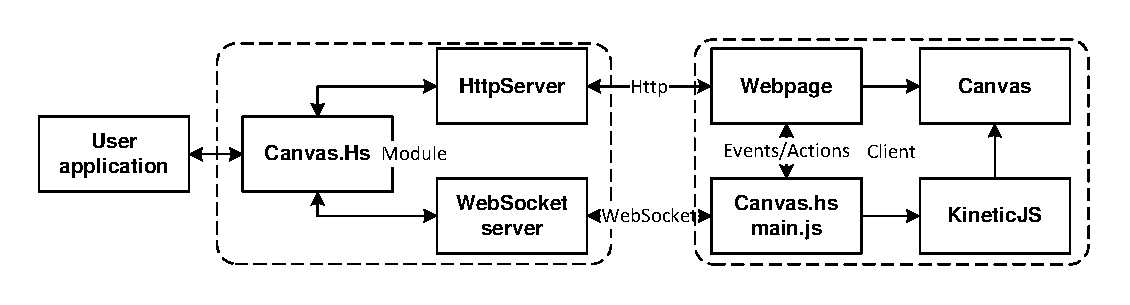
\includegraphics[keepaspectratio,width=\textwidth]{./images/architecture.pdf}
\caption{Architectuur van Canvas.hs}
\label{fig:architectuur}
\end{center}
\end{figure}

\subsubsection{Communicatie}
Gegevensoverdracht tussen de HTTP server en de browser moet snel gebeuren. Om de grafische elementen in de browser weer te geven moeten de output van de grafische interface naar de browser gecommuniceerd worden. Wanneer de gebruiker interactie heeft met de interface moet dit naar het programma van de gebruiker gecommuniceerd worden. Verder zal het programma bepaalde acties moeten kunnen uitvoeren op de webbrowser, zoals fullscreen laten gaan van de browser. Een belangrijke overwegingen is dat de grafische interface zo min mogelijk vertraging moet hebben.


\paragraph{Websockets}
Het is mogelijk om door middel van XMLHttpRequest of WebSockets een verbinding te onderhouden tussen de Module en de Clientomgeving. XMLHttpRequests worden door alle webbrowsers ondersteund, en kan door middel van longpolling technieken (Comet) \todo{PJ: wat is deze? of meer uitleg of verwijzingkje denk ik} een verbinding onderhouden met de webserver. De meest recente browsers ondersteunen WebSockets. Dit biedt een socket verbinding tussen de client en de server. Het WebSockets protocol biedt een betere performance dan alle technieken op basis van XMLHttpRequests en biedt een groter implementatiegemak. Door het gebruik van het HTML canvaselement zal de browser ondersteuning al beperkt zijn tot de meest recente browsers. Canvas.hs maakt gebruik van WebSockets.

\paragraph{Protocol}
In Cavas.hs wordt voor deze communicatie gebruik gemaakt van JSON \cite{JSON2006}. JSON staat voor JavaScript Object Notation en is een notatie waarin objecten als text worden gerepresenteerd zoals dit ook in Javascript wordt gedaan. JSON is een veel gebruikte notatie voor communicatie met Javascript. Het voordeel van JSON is, doordat het zo veel gebruikt wordt, dat er veel bibliotheken beschikbaar zijn om met JSON om te gaan. Zowel voor javascript als voor Haskell was het eenvoudig een goede externe bibliotheek te vinden om data van en naar JSON te lezen en te schrijven. Een ander groot voordeel van JSON is dat het, in tegenstelling tot bijvoorbeeld XML, weinig overhead heeft. Een uitgebreide handleiding van het protocol van gevonden worden in \cite{Protocol2013}.

Het protocol tussen de client en de server bevat voornamelijk interface data. De structuur en de attributen moeten vertaald worden van de Haskell omgeving om gebruikt te worden om te tekenen in het Canvas en vervolgens input van de gebruiker in de client te ondersteunen. De datastructuur van het protocol lijkt zoveel mogelijk op die van het canvas. Hierdoor kan data die binnenkomt bij de javascript applicatie zonder al te veel veranderingen op het canvas getekend worden.

\paragraph{Statelessness} \label{par:statelessness}
De Canvas.hs module houdt de huidige grafische boom niet bij. Deze wordt na ontvangst van de gebruiker applicatie onmiddelijk geëncodeerd naar JSON en opgestuurd naar de Javascriptapplicatie. Dit heeft een aantal voordelen. Allereerst maakt dit het gebruik van de module door de programmeur gemakkelijker. Elke keer dat de eventHandler wordt uitgevoerd wordt hiervan verwacht dat deze een volledige grafische boom oplevert waardoor het voor de programmeur en de module niet nodig is om uit te zoeken waar de grafische boom precies veranderd moet worden. Bijkomend voordeel hiervan is dat er slechts één plek is waar de huidige grafische boom wordt bijgehouden: de Javascriptapplicatie. Hierdoor kunnen er geen synchronisatiefouten tussen de Haskell module en de Javascriptapplicatie ontstaan. 

Nadeel van deze aanpak is dat er veel overhead is door het voortdurend versturen van de volledige grafische boom. Zelfs voor het verplaatsen van één object moet de hele boom opnieuw verstuurd worden. Dat er veel data verstuurd wordt is acceptabel aangezien het systeem ontwikkeld is voor lokaal gebruik en data over websockets lokaal zeer snel verstuurd kan worden. De aanpak levert echter wel problemen op als er snel veel getekend wordt, doordat het tekenen naar het canvas in onze aanpak relatief veel tijd kost. Hier wordt verder op gereflecteerd in \fullref{hoofdstuk:conclusie}.\todo{Dit daadwerkelijk doen.}